\chapter{पदार्थों की पहचान}\label{ch:g7:identifying-substances}

एक छोटे-से रहस्य की जगह पर काले फ़ेल्ट-पेन से लिखा एक मुड़ा-तुड़ा पर्चा
मिलता है, और तीन अलग-अलग थैलों में तीन फ़ेल्ट-पेन मिलते हैं। आँख को तीनों
स्याहियाँ एक जैसी काली दिखती हैं। एक न्यायालयिक रसायनज्ञ को यह बताने के लिए
कि पर्चा किस पेन से लिखा गया, बस कागज़ की एक पट्टी, थोड़ा पानी और आधा घंटा
चाहिए। रसायनज्ञ पदार्थों को इससे नहीं पहचानते कि वे कैसे दिखते हैं, बल्कि
इससे कि उनके लिए चुने गए परीक्षण में वे कैसा व्यवहार करते हैं।

\begin{recall}
\omterm{def:g6:pure-substances-and-mixtures:species}{रासायनिक स्पीशीज़} किसी पदार्थ का एक विशेष प्रकार है; \omterm{def:g6:pure-substances-and-mixtures:pure-substance}{शुद्ध पदार्थ} में केवल
एक स्पीशीज़ होती है, \omterm{def:g6:pure-substances-and-mixtures:mixture}{मिश्रण} में कई
(\cref{ch:g6:pure-substances-and-mixtures})। कुछ पदार्थ किसी \omterm{def:g6:solutions-and-solubility:solute}{विलायक} में
अच्छी तरह \omterm{def:g2:mixing-and-dissolving:dissolve}{घुलते} हैं, कुछ थोड़ा या बिल्कुल नहीं: हर एक की अपनी
\omterm{def:g6:solutions-and-solubility:solubility}{विलेयता} होती है (\cref{ch:g6:solutions-and-solubility})।
\end{recall}

\section{अभिलाक्षणिक परीक्षण क्या है}

\begin{definition}[अभिलाक्षणिक परीक्षण और अभिकर्मक]\label{def:g7:identifying-substances:characteristic-test}
किसी \omterm{def:g6:pure-substances-and-mixtures:species}{रासायनिक स्पीशीज़} का \emph{अभिलाक्षणिक परीक्षण}\index{अभिलाक्षणिक परीक्षण}
एक सरल प्रयोग है जो उस स्पीशीज़ के साथ एक दिखाई देने वाला परिणाम देता है,
और उसी स्थिति में मिलने वाली दूसरी स्पीशीज़ के साथ नहीं। इसमें इसी काम के
लिए चुना गया एक पदार्थ इस्तेमाल होता है, जिसे
\emph{अभिकर्मक}\index{अभिकर्मक} कहते हैं।
\end{definition}


\begin{method}[अभिलाक्षणिक परीक्षण करना]\label{met:g7:identifying-substances:run}
\begin{enumerate}
  \item परखे जाने वाले पदार्थ का एक छोटा नमूना लो।
  \item परीक्षण में बताए अनुसार \omterm{def:g7:identifying-substances:characteristic-test}{अभिकर्मक} मिलाओ, या उसे नमूने के संपर्क
        में लाओ।
  \item प्रेक्षण करो: रंग का बदलना, धुँधलापन, कोई लौ, कोई आवाज़।
  \item निष्कर्ष निकालो: अपेक्षित परिणाम दिखे तो परीक्षण \emph{धनात्मक}
        है, न दिखे तो \emph{ऋणात्मक}।
  \item वही परीक्षण ऐसे नमूने पर भी करो जिसमें वह स्पीशीज़ निश्चित रूप से
        न हो (रिक्त परीक्षण): वह ऋणात्मक ही रहना चाहिए, वरना परिणाम कुछ
        सिद्ध नहीं करता।
\end{enumerate}
\end{method}

\section{चार प्रसिद्ध परीक्षण}

\begin{proposition}[कार्बन डाइऑक्साइड चूने के पानी को दूधिया कर देती है]\label{prop:g7:identifying-substances:limewater}
चूने का पानी एक स्वच्छ, रंगहीन विलयन है। जब उसमें से कार्बन डाइऑक्साइड के
बुलबुले गुज़ारे जाते हैं, तो वह दूधिया, धुँधला सफ़ेद हो जाता है। स्ट्रॉ से
बाहर छोड़ी गई साँस चूने के पानी को दूधिया कर देती है; उसमें से पंप की गई
ताज़ी \omterm{def:g4:air-a-mixture-of-gases:air}{हवा} मुश्किल से ही ऐसा करती है।
\end{proposition}

\begin{omfigure}
\begin{tikzpicture}[font=\small, scale=1.25]
  % generating tube, stoppered
  \pic[transform shape] at (0,0) {testtube={0.35}{omWater!80}};
  \fill[black!65] (-0.27,2.8) rectangle (0.27,3.15);
  \foreach \y in {0.4,0.65,0.85} \draw[black!55] (0.05,\y) circle (0.04);
  \pic[transform shape] at (0,2.9) {deliverytube={1.9}{-2.3}};
  % limewater tube
  \pic[transform shape] at (1.9,0) {testtube={0.6}{white!85!black}};
  \foreach \x/\y in {1.88/0.75,1.95/1.0,1.85/1.25,1.92/1.5} \draw[black!55] (\x,\y) circle (0.04);
  \draw[<-, omProp, thick] (-0.3,0.5) -- (-1.2,0.8) node[left, text=black, align=right]
    {गैस देने वाली\\ एक अभिक्रिया};
  \draw[<-, omProp, thick] (2.2,1.2) -- (3.0,1.4) node[right, text=black, align=left]
    {चूने का पानी दूधिया\\ होता है: गैस कार्बन\\ डाइऑक्साइड है};
\end{tikzpicture}

{\small चूने के पानी का परीक्षण। पहली नली में निकलने वाली गैस चूने के पानी
में से बुलबुलों के रूप में गुज़रती है; अगर चूने का पानी दूधिया हो जाए, तो
गैस कार्बन डाइऑक्साइड है।}
\end{omfigure}

\begin{proposition}[पानी निर्जल कॉपर सल्फ़ेट को नीला कर देता है]\label{prop:g7:identifying-substances:copper-sulfate}
निर्जल कॉपर सल्फ़ेट एक सफ़ेद चूर्ण है। पानी की एक बूँद उसे तुरंत नीला
कर देती है। यह परीक्षण दिखाता है कि किसी द्रव या नम ठोस में पानी मौजूद
है --- यह नहीं कि वह द्रव शुद्ध पानी है।
\end{proposition}

\begin{omfigure}
\begin{minipage}[b]{0.48\linewidth}\centering
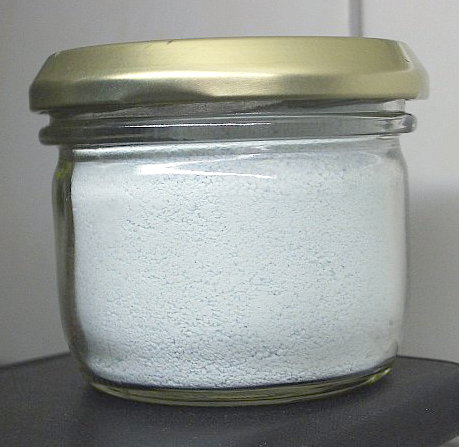
\includegraphics[width=\linewidth,height=4.2cm,keepaspectratio]{images/book1/cuso4-anhydrous.jpg}

{\small निर्जल कॉपर सल्फ़ेट: एक सफ़ेद चूर्ण। फ़ोटो: डब्ल्यू.~ओलेन,
CC BY-SA 3.0।}
\end{minipage}\hfill
\begin{minipage}[b]{0.48\linewidth}\centering
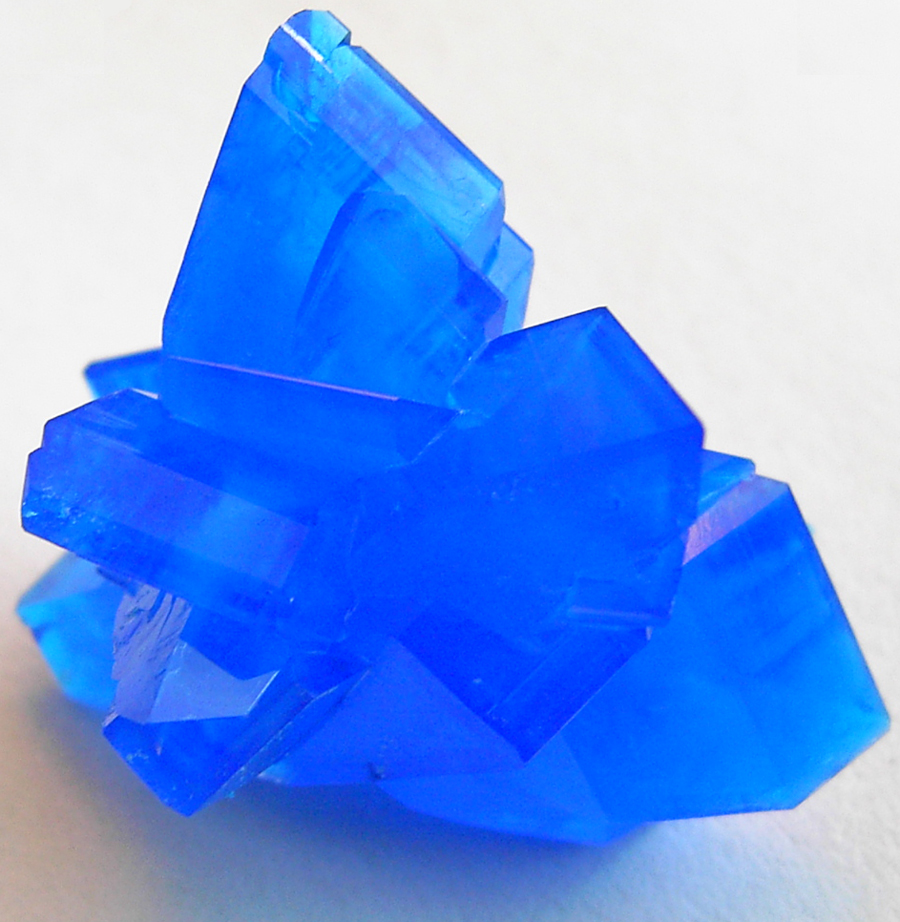
\includegraphics[width=\linewidth,height=4.2cm,keepaspectratio]{images/book1/cuso4-hydrated.jpg}

{\small पानी के साथ यह नीला हो जाता है; इन क्रिस्टलों में पानी है। फ़ोटो:
स्टेफ़ानबी, CC BY-SA 3.0।}
\end{minipage}
\end{omfigure}

\begin{safety}{\ghs[0.82cm]{GHS05}\ghs[0.82cm]{GHS07}\ghs[0.82cm]{GHS09}}
% ledger: ghs:CuSO4
कॉपर सल्फ़ेट: निगलने पर हानिकारक और त्वचा में जलन करने वाला (GHS07);
यह आँखों को गंभीर हानि पहुँचा सकता है (GHS05); जलीय जीवों के लिए अत्यंत
विषैला, लंबे समय तक रहने वाले प्रभावों के साथ (GHS09)। चश्मा और दस्ताने
ज़रूरी; अपशिष्ट इकट्ठा किया जाता है, कभी नाली में नहीं बहाया जाता।
\end{safety}

\begin{proposition}[ऑक्सीजन सुलगती खपच्ची को फिर जला देती है]\label{prop:g7:identifying-substances:splint}
लकड़ी की एक खपच्ची \omterm{def:g4:what-a-fire-needs:burning}{जलाई} जाती है, फिर फूँककर बुझाई जाती है ताकि केवल एक
लाल सुलगन बचे। ऑक्सीजन से भरी परखनली में डालने पर सुलगती खपच्ची फिर से
लौ पकड़ लेती है।
\end{proposition}

\begin{proposition}[हाइड्रोजन `पॉप' की तीखी आवाज़ के साथ जलती है]\label{prop:g7:identifying-substances:pop}
हाइड्रोजन से भरी एक छोटी परखनली के मुँह पर पकड़ी गई \omterm{def:g4:what-a-fire-needs:burning}{जलती} खपच्ची एक छोटी,
तीखी ``पॉप'' की आवाज़ करती है: हाइड्रोजन \omterm{def:g4:air-a-mixture-of-gases:air}{वायु} की ऑक्सीजन के साथ तुरंत
जल जाती है।
\end{proposition}

\begin{omfigure}
\begin{tikzpicture}[font=\small, scale=1.25]
  % splint test for oxygen
  \pic[transform shape] at (0,0) {testtube={0}{white}};
  \draw[brown!60!black, line width=2pt] (0.15,1.6) -- (1.4,3.6);
  \fill[orange!85] (0.15,1.6) circle (0.07);
  \fill[orange!80] (0.12,1.62) .. controls (0.0,1.9) and (0.08,2.1) .. (0.1,2.3)
    .. controls (0.2,2.05) and (0.3,1.85) .. (0.2,1.62);
  \node[anchor=north, align=center] at (0,-0.15) {ऑक्सीजन:\\ सुलगती खपच्ची\\ लौ पकड़ लेती है};
  % pop test for hydrogen
  \begin{scope}[xshift=4cm]
    \pic[transform shape, rotate=180] at (0,3.1) {testtube={0}{white}};
    \draw[brown!60!black, line width=2pt] (0.05,-0.05) -- (1.3,-0.9);
    \fill[orange!85] (0.05,-0.02) .. controls (-0.05,0.08) and (0.0,0.15) .. (0.02,0.22)
      .. controls (0.08,0.15) and (0.15,0.08) .. (0.1,-0.02);
    \node[font=\small\itshape] at (-0.9,0.15) {पॉप!};
    \node[anchor=north, align=center] at (0,-1.0) {हाइड्रोजन:\\ मुँह पर तीखी\\ `पॉप' की आवाज़};
  \end{scope}
\end{tikzpicture}

{\small बाएँ: सुलगती खपच्ची ऑक्सीजन में फिर जल उठती है। दाएँ: हाइड्रोजन से भरी
उलटी नली के मुँह पर \omterm{def:g4:what-a-fire-needs:burning}{जलती} खपच्ची तीखी `पॉप' की आवाज़ करती है
(हाइड्रोजन \omterm{def:g4:air-a-mixture-of-gases:air}{वायु} से हल्की है, इसलिए नली मुँह नीचे करके पकड़ी जाती है)।}
\end{omfigure}

\begin{safety}{\ghs[0.82cm]{GHS02}\ghs[0.82cm]{GHS04}}
% ledger: ghs:H2
हाइड्रोजन: अत्यंत ज्वलनशील गैस (GHS02), सिलिंडरों में दाब के साथ रखी
जाती है (GHS04)। `पॉप' परीक्षण केवल कुछ मिलीलीटर गैस से, शिक्षक द्वारा,
किया जाता है।
\end{safety}

\section{पेपर वर्णलेखन}

\begin{definition}[पेपर वर्णलेखन और वर्णलेख]\label{def:g7:identifying-substances:chromatography}
\emph{पेपर वर्णलेखन}\index{पेपर वर्णलेखन} किसी \omterm{def:g6:pure-substances-and-mixtures:mixture}{मिश्रण} के रंजकों को अलग
करता है। कागज़ की एक पट्टी के निचले सिरे के पास खींची गई रेखा पर \omterm{def:g6:pure-substances-and-mixtures:mixture}{मिश्रण} का
एक छोटा धब्बा लगाया जाता है; पट्टी का निचला सिरा एक \omterm{def:g6:solutions-and-solubility:solute}{विलायक} में डूबा होता
है, जो धीरे-धीरे कागज़ पर ऊपर चढ़ता है और हर रंजक को अपने साथ ले जाता है,
कुछ को दूसरों से तेज़। जब \omterm{def:g6:solutions-and-solubility:solute}{विलायक} लगभग ऊपर तक चढ़ जाता है, तो पट्टी निकालकर
सुखाई जाती है: यही
\emph{वर्णलेख}\index{वर्णलेख} है।
\end{definition}

\begin{omfigure}
\begin{tikzpicture}[font=\small, scale=1.3]
  % the strip in a beaker of solvent
  \pic[transform shape] at (0,0) {beaker={0.12}{omWater!80}};
  \fill[white] (-0.42,0.06) rectangle (0.42,2.2);
  \fill[omWater!80] (-0.42,0.06) rectangle (0.42,0.24);
  \draw[omGlass, line width=0.6pt] (-0.42,0.06) rectangle (0.42,2.2);
  \draw[black!60, line width=0.4pt] (-0.42,0.42) -- (0.42,0.42);
  \fill[black!80] (0,0.42) circle (0.07);
  \shade[ball color=black!20] (0,2.27) circle (0.08);
  \draw[black!50, line width=1.2pt] (-1.1,2.27) -- (1.1,2.27);
  \node[anchor=north, align=center] at (0,-0.15) {शुरुआत में};
  \draw[<-, omProp, thick] (0.1,0.5) -- (1.3,0.8) node[right, text=black]
    {पेंसिल की रेखा पर स्याही का धब्बा};
  \draw[<-, omProp, thick] (1.0,2.27) -- (1.3,2.5) node[right, text=black]
    {कागज़ को थामे काँच की छड़};
  \draw[<-, omProp, thick] (0.75,0.15) -- (1.3,0.25) node[right, text=black]
    {विलायक, रेखा के नीचे};
  % the chromatogram
  \begin{scope}[xshift=6.2cm]
    \pic[transform shape] at (0,0) {tlcplate};
    \draw[black!50, dashed] (-0.7,2.7) -- (0.7,2.7);
    \fill[blue!70] (0,1.0) ellipse (0.13 and 0.09);
    \fill[red!70] (0,1.7) ellipse (0.13 and 0.09);
    \fill[yellow!80!orange] (0,2.35) ellipse (0.13 and 0.09);
    \node[anchor=north, align=center] at (0,-0.15) {वर्णलेख};
    \draw[<-, omProp, thick] (0.75,2.7) -- (1.3,2.85) node[right, text=black]
      {विलायक कहाँ तक चढ़ा};
    \draw[<-, omProp, thick] (0.2,1.7) -- (1.3,1.7) node[right, text=black]
      {तीन रंजक: स्याही एक मिश्रण है};
  \end{scope}
\end{tikzpicture}

{\small काली स्याही का \omterm{def:g7:identifying-substances:chromatography}{पेपर वर्णलेखन}। \omterm{def:g6:solutions-and-solubility:solute}{विलायक} कागज़ में ऊपर चढ़ता है और
स्याही को तीन रंजकों में अलग कर देता है।}
\end{omfigure}

\begin{method}[वर्णलेख पढ़ना]\label{met:g7:identifying-substances:read}
\begin{enumerate}
  \item हर प्रारंभ-बिंदु के ऊपर धब्बे गिनो: एक धब्बा, एक रंजक; दो या
        ज़्यादा धब्बे, रंजकों का \omterm{def:g6:pure-substances-and-mixtures:mixture}{मिश्रण}।
  \item ऊँचाइयों की तुलना करो: एक ही \omterm{def:g7:identifying-substances:chromatography}{वर्णलेख} में एक रंजक हमेशा उतनी ही
        ऊँचाई तक चढ़ता है। किसी ज्ञात रंजक जितनी ऊँचाई वाला धब्बा शायद वही
        रंजक है।
  \item पेंसिल की रेखा बनाओ, स्याही की कभी नहीं: \omterm{def:g6:solutions-and-solubility:solute}{विलायक} ख़ुद उस स्याही को भी
        अलग कर देगा।
\end{enumerate}
\end{method}

\begin{example}[टॉफ़ियों के रंजक]\label{ex:g7:identifying-substances:sweets}
टॉफ़ियों की रंगीन परतें खुरचकर थोड़े पानी में डाली जाती हैं और पट्टी पर
धब्बों के रूप में लगाई जाती हैं, टॉफ़ियों में अनुमत खाद्य रंजकों के धब्बों के
बगल में। \omterm{def:g7:identifying-substances:chromatography}{वर्णलेख} दिखाता है कि हरी परत में एक पीला और एक नीला रंजक है,
और दोनों अनुमत रंजकों में शामिल हैं।
\end{example}


\section{परीक्षण-सारणी पढ़ना}

\begin{proposition}[अभिलाक्षणिक परीक्षणों की एक सारणी]\label{prop:g7:identifying-substances:bank}
रसायनज्ञ अपने परीक्षणों को एक सारणी में रखते हैं, जिसे परीक्षण-सारणी कहते हैं
और जो बाएँ से दाएँ पढ़ी जाती है:
\begin{center}
\small
\begin{tabular}{llll}
\hline
खोजी जाने वाली स्पीशीज़ & \omterm{def:g7:identifying-substances:characteristic-test}{अभिकर्मक} या परीक्षण & धनात्मक परिणाम & \\
\hline
कार्बन डाइऑक्साइड & चूने का पानी & चूने का पानी दूधिया होता है & \\
पानी & निर्जल कॉपर सल्फ़ेट & सफ़ेद से नीला & \\
ऑक्सीजन & सुलगती खपच्ची & खपच्ची फिर जल उठती है & \\
हाइड्रोजन & \omterm{def:g4:what-a-fire-needs:burning}{जलती} खपच्ची & तीखी `पॉप' & \\
\omterm{def:g6:pure-substances-and-mixtures:mixture}{मिश्रण} के रंजक & \omterm{def:g7:identifying-substances:chromatography}{पेपर वर्णलेखन} & हर रंजक का एक धब्बा & \\
\hline
\end{tabular}
\end{center}
\end{proposition}

\begin{remark}[परीक्षण क्या नहीं बताता]\label{rem:g7:identifying-substances:limits}
धनात्मक परीक्षण यह सिद्ध करता है कि स्पीशीज़ मौजूद है, यह नहीं कि वह अकेली
है: कॉपर सल्फ़ेट को नीला करने वाले द्रव में पानी है, पर वह नमकीन पानी या
संतरे का रस भी हो सकता है। ऋणात्मक परीक्षण बस इतना बताता है कि स्पीशीज़
मौजूद नहीं है, या इतनी कम मात्रा में है कि दिखती नहीं।
\end{remark}

\begin{omfigure}
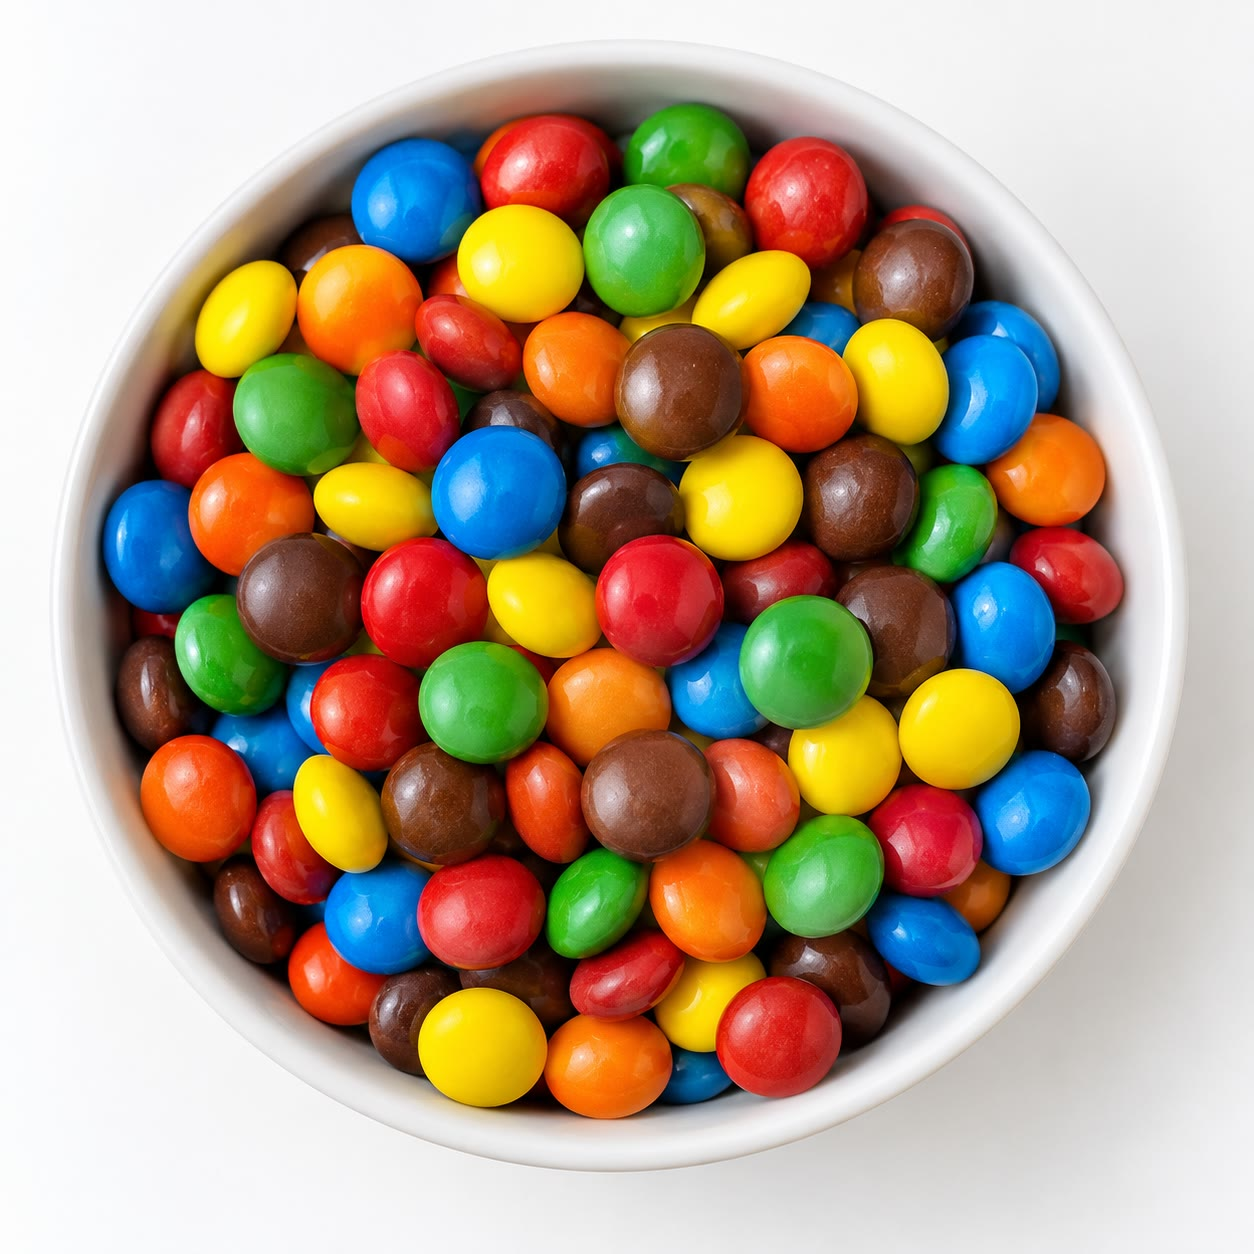
\includegraphics[width=0.32\linewidth]{images/book1/ai/g7-sweets.jpg}

{\small चीनी चढ़ी टॉफ़ियाँ: उनके रंग रंजकों के \omterm{def:g6:pure-substances-and-mixtures:mixture}{मिश्रण} हैं, जिन्हें
वर्णलेखन अलग कर सकता है।}
\end{omfigure}

\begin{omfigure}
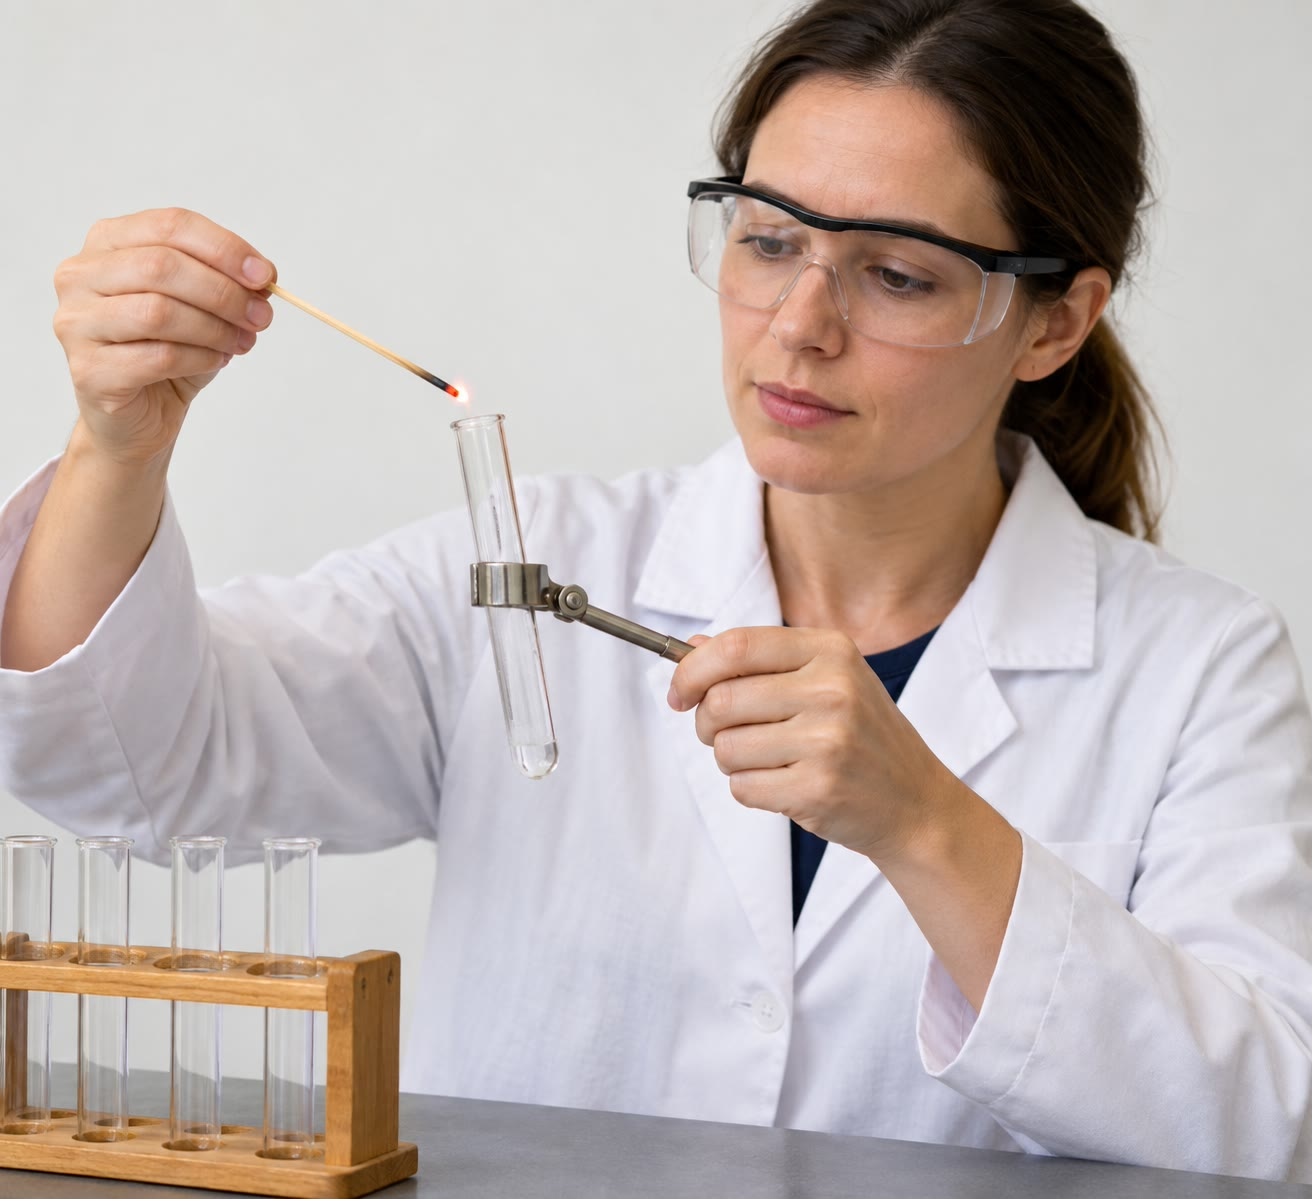
\includegraphics[width=0.36\linewidth]{images/book1/ai/g7-splint-teacher.jpg}

{\small शिक्षक सुलगती खपच्ची से एक गैस का परीक्षण करते हैं।}
\end{omfigure}

\section{अभ्यास}

\begin{exercise}[$\star$]\label{exo:g7:identifying-substances:1}
कौन-सा परीक्षण कार्बन डाइऑक्साइड को पहचानता है? उसके धनात्मक परिणाम का वर्णन करो।
\end{exercise}

\begin{exercise}[$\star$]\label{exo:g7:identifying-substances:2}
एक सफ़ेद चूर्ण पर कोई द्रव टपकाने से वह नीला हो जाता है। इससे द्रव के
बारे में क्या पता चलता है?
\end{exercise}

\begin{exercise}[$\star$]\label{exo:g7:identifying-substances:3}
सुलगती खपच्ची गैस-जार में डालने पर लौ पकड़ लेती है। जार में कौन-सी गैस
है?
\end{exercise}

\begin{exercise}[$\star$]\label{exo:g7:identifying-substances:4}
पेपर \omterm{def:g7:identifying-substances:chromatography}{वर्णलेख} की प्रारंभ-रेखा पेंसिल से क्यों खींची जाती है,
स्याही से क्यों नहीं?
\end{exercise}

\begin{exercise}[$\star\star$]\label{exo:g7:identifying-substances:5}
प्रारंभ-रेखा बीकर में \omterm{def:g6:solutions-and-solubility:solute}{विलायक} के तल से ऊपर क्यों होनी
चाहिए?
\end{exercise}

\begin{exercise}[$\star\star$]\label{exo:g7:identifying-substances:6}
हरी स्याही के \omterm{def:g7:identifying-substances:chromatography}{वर्णलेख} में दो धब्बे दिखते हैं, एक पीले संदर्भ रंजक की ऊँचाई
पर, एक नीले संदर्भ रंजक की ऊँचाई पर। क्या हरी स्याही एक \omterm{def:g6:pure-substances-and-mixtures:pure-substance}{शुद्ध पदार्थ} है?
वह किससे बनी है?
\end{exercise}

\begin{exercise}[$\star\star$]\label{exo:g7:identifying-substances:7}
परीक्षण-सारणी की मदद से बताओ कि यह दिखाने के लिए कि किसी अभिक्रिया से निकली
गैस हाइड्रोजन है, तुम कौन-सा परीक्षण करोगे। तुम क्या देखने की अपेक्षा करते हो?
\end{exercise}

\begin{exercise}[$\star\star$]\label{exo:g7:identifying-substances:8}
बाहर छोड़ी गई साँस ताज़ी \omterm{def:g4:air-a-mixture-of-gases:air}{हवा} की तुलना में चूने के पानी को कहीं जल्दी दूधिया
कर देती है। इससे हमारी बाहर छोड़ी गई साँस के बारे में क्या पता चलता है?
\end{exercise}

\begin{exercise}[$\star\star$]\label{exo:g7:identifying-substances:9}
एक स्वच्छ द्रव निर्जल कॉपर सल्फ़ेट को नीला कर देता है। सैम निष्कर्ष निकालता
है: ``यह शुद्ध पानी है।'' समझाओ कि सैम ग़लत क्यों है।
\end{exercise}

\begin{exercise}[$\star\star$]\label{exo:g7:identifying-substances:10}
इस अध्याय में काली स्याही का \omterm{def:g7:identifying-substances:chromatography}{वर्णलेख} देखो। स्याही में कितने रंजक हैं?
कौन-सा सबसे ऊपर चढ़ा?
\end{exercise}

\begin{exercise}[$\star\star\star$]\label{exo:g7:identifying-substances:11}
तीन जारों में ऑक्सीजन, हाइड्रोजन और कार्बन डाइऑक्साइड हैं, पर उनके लेबल खो
गए हैं। कागज़ पर उन परीक्षणों की योजना बनाओ जो हर जार की गैस का नाम बता दें,
ऐसे क्रम में कि कम से कम परीक्षण लगें।
\end{exercise}

\begin{exercise}[$\star\star\star$]\label{exo:g7:identifying-substances:12}
एक छात्र चूने के पानी से एक गैस का परीक्षण करता है और कुछ होता नहीं देखता।
दो संभव कारण बताओ, और वह नियंत्रण परीक्षण भी जो फ़ैसला करने में मदद करे।
\end{exercise}

\section{समस्या: जाली पर्चा}

\begin{problem}[{सप्ताहांत समस्या --- फ़ेल्ट-पेन से लिखा एक पर्चा, तीन संदिग्ध पेन,
तीन बिना लेबल के गैस-सिलिंडर, और एक परीक्षण-सारणी}]
\label{pb:g7:identifying-substances:1}
एक विद्यालय की प्रयोगशाला से दो छोटे रहस्य सुलझाने में मदद माँगी जाती है।
पहला, काले फ़ेल्ट-पेन से लिखे एक पर्चे को तीन काले पेनों 1, 2 और 3 में से
किसी एक से मिलाना है। पर्चे से और हर पेन से स्याही की एक बूँद लेकर कागज़ की
एक ही पट्टी पर धब्बे लगाए जाते हैं, फिर पट्टी को पानी से विकसित किया जाता है।
\omterm{def:g7:identifying-substances:chromatography}{वर्णलेख} नीचे दिखाया गया है।
\begin{center}
\begin{tikzpicture}[font=\small, x=1cm, y=1cm]
  \fill[white] (0,0) rectangle (6,4);
  \draw[omGlass, line width=0.6pt] (0,0) rectangle (6,4);
  \draw[black!60] (0,0.5) -- (6,0.5);
  \draw[black!50, dashed] (0,3.6) -- (6,3.6);
  \foreach \x/\lab in {0.9/पर्चा, 2.3/पेन 1, 3.7/पेन 2, 5.1/पेन 3}
    \node[anchor=north] at (\x,-0.05) {\lab};
  % note: three dyes
  \fill[blue!70] (0.9,1.2) ellipse (0.18 and 0.1);
  \fill[red!70] (0.9,2.2) ellipse (0.18 and 0.1);
  \fill[yellow!80!orange] (0.9,3.1) ellipse (0.18 and 0.1);
  % pen 1: two dyes
  \fill[blue!70] (2.3,1.2) ellipse (0.18 and 0.1);
  \fill[black!70] (2.3,2.7) ellipse (0.18 and 0.1);
  % pen 2: same three as the note
  \fill[blue!70] (3.7,1.2) ellipse (0.18 and 0.1);
  \fill[red!70] (3.7,2.2) ellipse (0.18 and 0.1);
  \fill[yellow!80!orange] (3.7,3.1) ellipse (0.18 and 0.1);
  % pen 3: three dyes, other heights
  \fill[violet!70] (5.1,0.9) ellipse (0.18 and 0.1);
  \fill[red!70] (5.1,1.8) ellipse (0.18 and 0.1);
  \fill[green!60!black] (5.1,2.6) ellipse (0.18 and 0.1);
  \node[anchor=west, font=\footnotesize] at (6.1,3.6) {विलायक अग्र};
  \node[anchor=west, font=\footnotesize] at (6.1,0.5) {प्रारंभ-रेखा};
\end{tikzpicture}
\end{center}

\medskip
\noindent\textbf{भाग I --- \omterm{def:g7:identifying-substances:chromatography}{वर्णलेख}।}
\begin{enumerate}
  \item चारों स्याहियों के धब्बे एक ही पट्टी पर क्यों लगाए गए और उन्हें एक
        साथ क्यों विकसित किया गया?
  \item पर्चे की स्याही \omterm{def:g6:pure-substances-and-mixtures:pure-substance}{शुद्ध पदार्थ} है या \omterm{def:g6:pure-substances-and-mixtures:mixture}{मिश्रण}? समझाओ।
  \item पेन 1 की स्याही में कितने रंजक हैं? क्या पर्चा पेन 1 से लिखा गया
        हो सकता है?
  \item पेन 3 में भी तीन रंजक हैं। वह पर्चा क्यों नहीं लिख सकता
        था?
  \item कौन-सा पेन पर्चे से मेल खाता है? धब्बों की ऊँचाइयों की मदद से
        समझाओ।
\end{enumerate}

\medskip
\noindent\textbf{भाग II --- तीन गैस-सिलिंडर।}
दूसरा रहस्य: तीन छोटे सिलिंडरों X, Y और Z के लेबल खो गए हैं; उनमें
ऑक्सीजन, हाइड्रोजन और कार्बन डाइऑक्साइड हैं। हर एक से थोड़ी गैस एक परखनली
में इकट्ठी की जाती है। गैस X सुलगती खपच्ची को फिर जला देती है। गैस Y \omterm{def:g4:what-a-fire-needs:burning}{जलती}
खपच्ची के साथ तीखी `पॉप' की आवाज़ करती है। गैस Z चूने के पानी को दूधिया कर देती है।
\begin{enumerate}[resume]
  \item गैस X का नाम बताओ।
  \item गैस Y का नाम बताओ।
  \item गैस Z का नाम बताओ।
  \item गैस Z का परीक्षण करने से पहले छात्र उसी चूने के पानी में से उतनी ही
        देर साधारण \omterm{def:g4:air-a-mixture-of-gases:air}{हवा} गुज़ारता है, और वह स्वच्छ रहता है। इस दूसरे परीक्षण
        को क्या कहते हैं, और यह निष्कर्ष में क्या जोड़ता है?
\end{enumerate}

\medskip
\noindent\textbf{भाग III --- परीक्षण-सारणी।}
\begin{enumerate}[resume]
  \item पर्चे के पास मिला एक रंगहीन द्रव निर्जल कॉपर सल्फ़ेट को नीला कर देता
        है। परीक्षण-सारणी की इस्तेमाल हुई पंक्ति लिखो, और बताओ कि परिणाम
        क्या दिखाता है।
  \item क्या यह परिणाम सिद्ध करता है कि द्रव शुद्ध पानी है? समझाओ।
  \item पहले रहस्य का निष्कर्ष निकालो: पर्चे की स्याही में कितने रंजक हैं,
        और उसे किस पेन ने लिखा?
\end{enumerate}
\end{problem}
